\chapter{Metodología}

En este capítulo describimos en profundidad todos los pasos seguidos en los métodos empleados en el trabajo y su justificación. Posteriormente, se aplicarán en la experimentación.

\section{Análisis de los recursos disponibles}

Para la realización de este trabajo debemos considerar los recursos hardware disponibles para la inferencia de los modelos pero sobre todo para el entrenamiento de los modelos.

\begin{enumerate}
	\item \textbf{Hardware en entrenamiento}. Para el desarrollo de toda la experimentación, entrenamiento de los modelos y validación nos valdremos de los recursos que gratuitamente ofrece Kaggle, una plataforma de ciencia de datos propiedad de Google. 
	
	El recurso más importante que ofrece Kaggle y razón de su uso es que nos permite el uso de su gráfica NVIDIA Tesla P100 por 30 horas semanales. Con ella, podemos entrenar los modelos y hacer una inferencia rápida para validación en tiempo razonable.
	
	Por nosotros mismos sólo disponíamos de un ordenador personal que aunque con mejor disponibilidad de memoria en disco $\approx 2\ TB$ que la ofrecida por Kaggle $\approx 100\ GB$, nuestra gráfica NVIDIA GeForce RTX 2060 tiene inmensamente menores prestaciones que la ofrecida en Kaggle. A continuación, mostramos una gráfica de rendimiento sobre las características de ambos dispositivos para cuantificar este hecho.
	
	\begin{figure}[H]
		\centering
		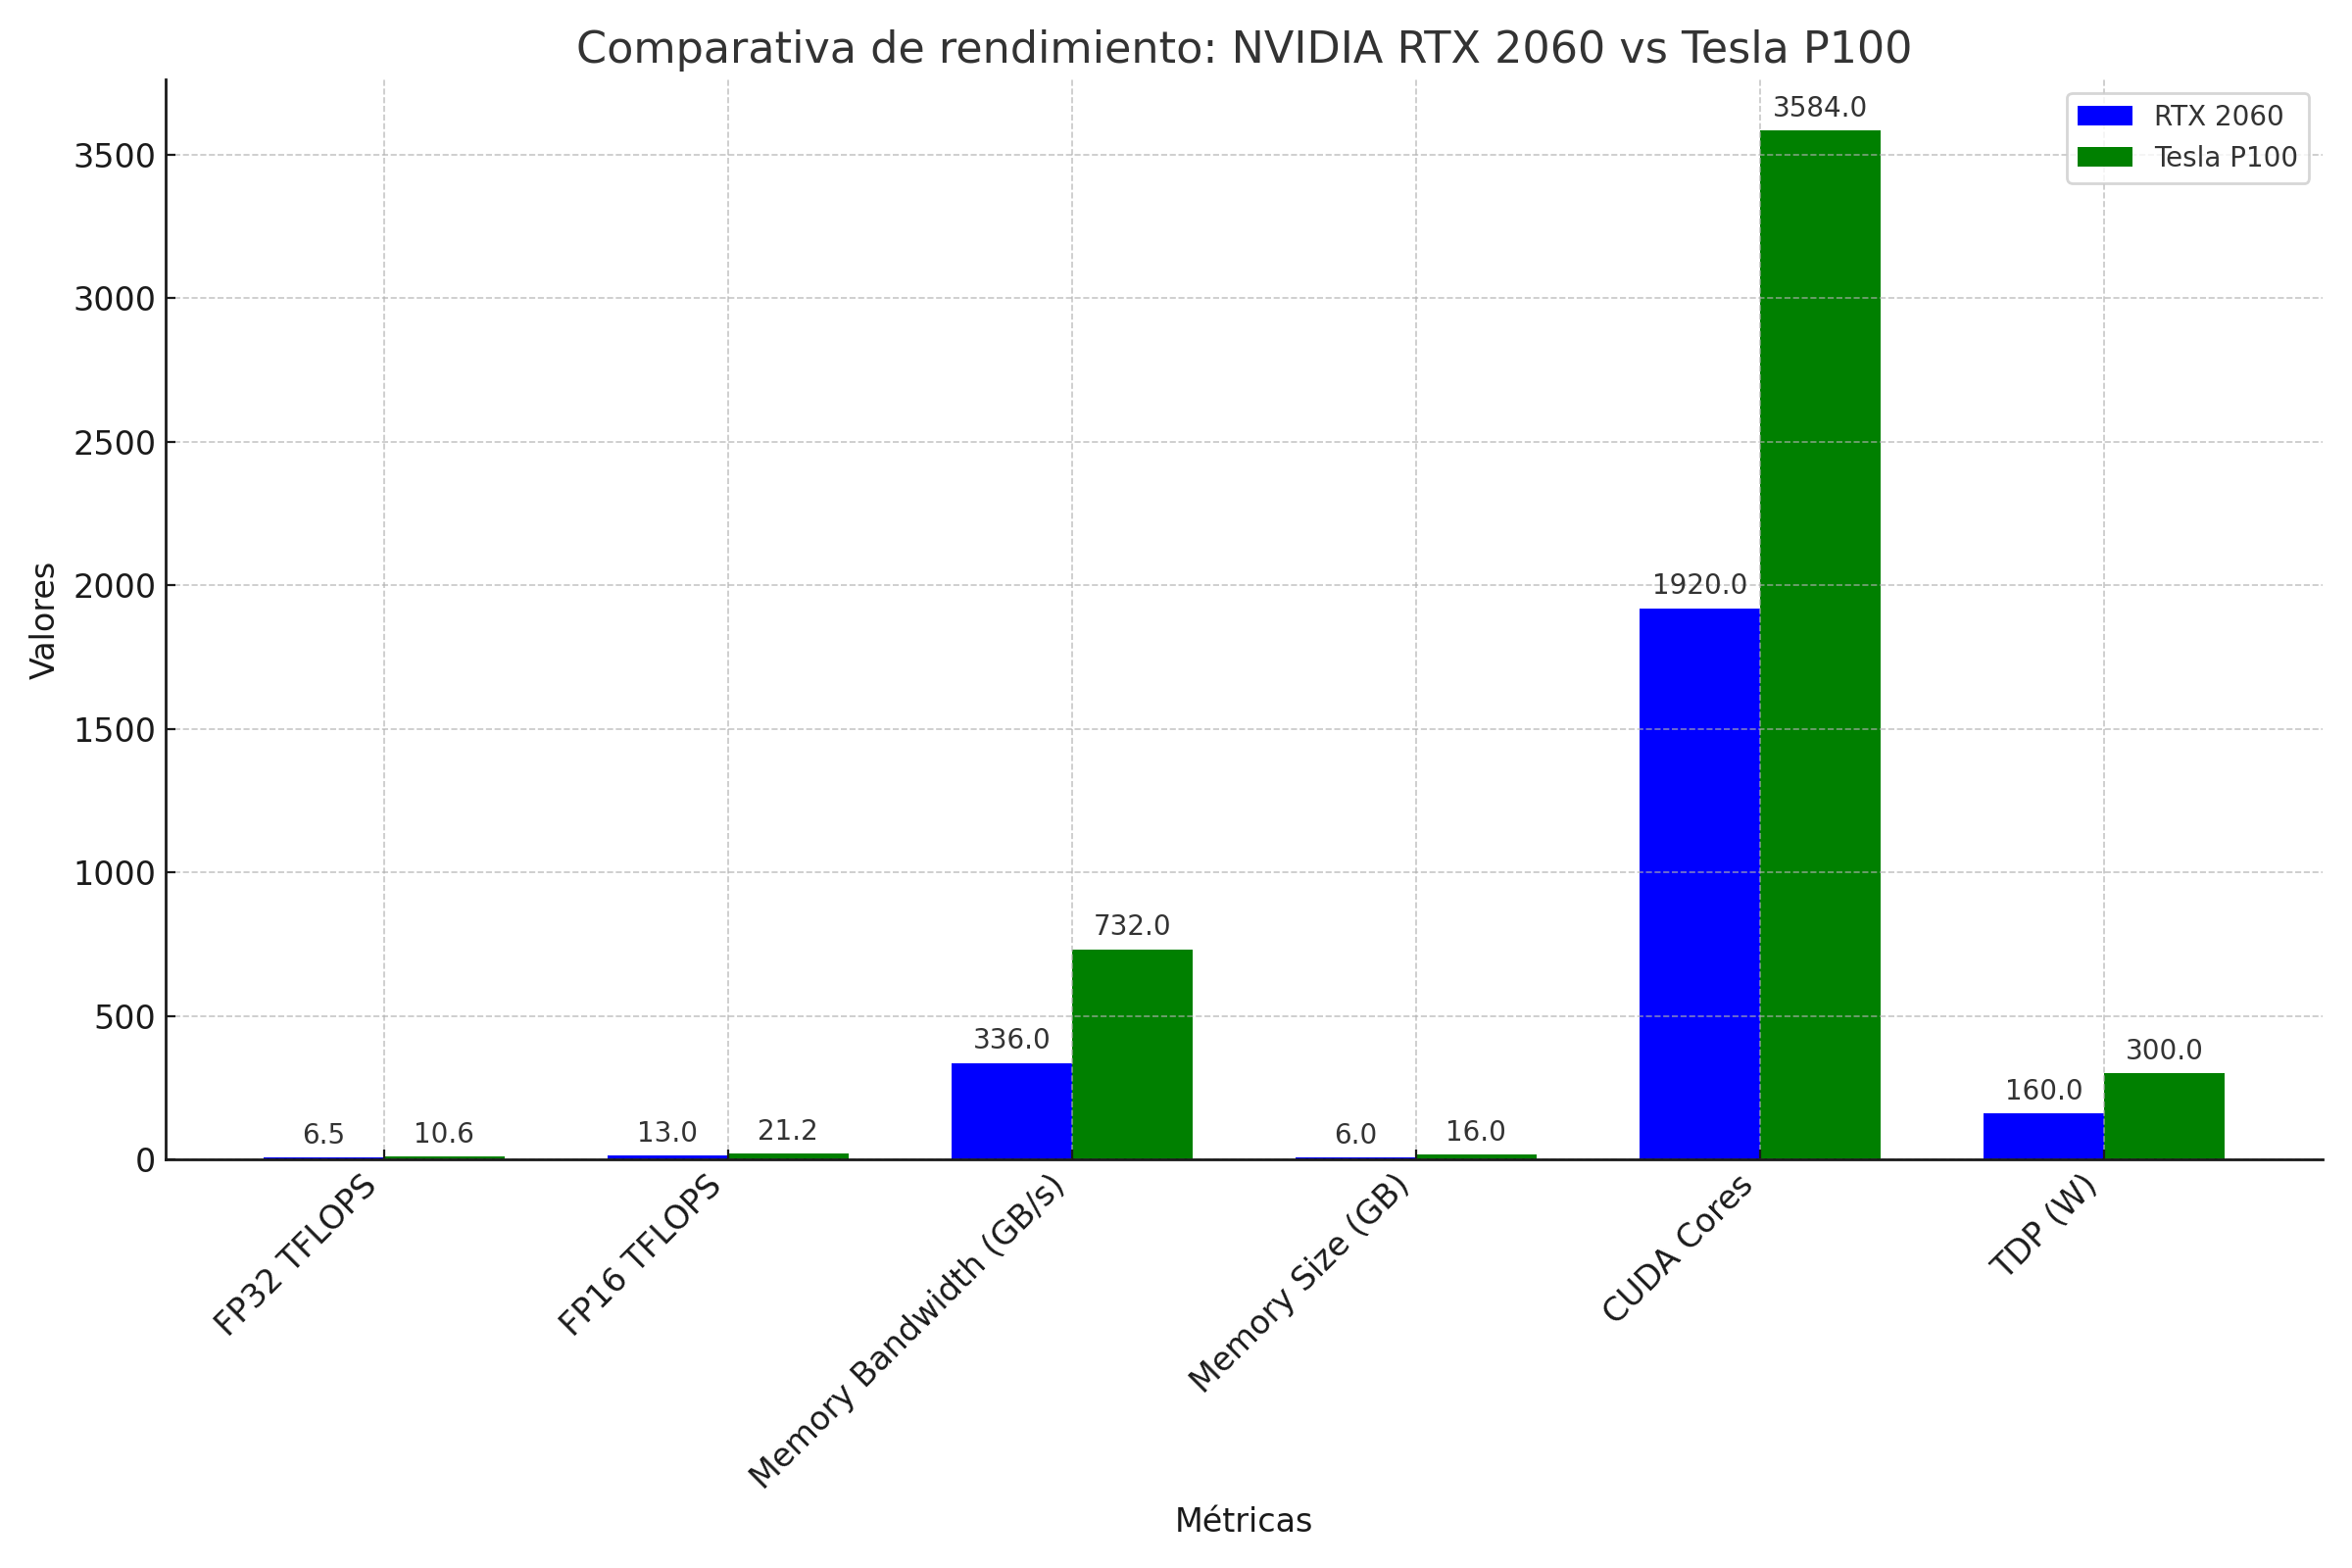
\includegraphics[width=1.0\linewidth]{imagenes/comparativa_rtx2060tesla.png}
		\caption{Comparativa de rendimiento de las GPU disponibles}
	\end{figure}
	
	
	\item \textbf{Hardware para inferir con los modelos}. De forma general, cualquier PC de uso personal que disponga de una GPU de rendimiento igual o mayor que   y cumpla las siguientes dependencias (link a apéndice de uso del programa). 
\end{enumerate}


\section{Preprocesado de Datos}

En este apartado se explicará el preprocesamiento que se ha aplicado a las resonancias magnéticas para convertirlas a entradas de los modelos. 

Partiendo de nuestro conjunto de datos que presentamos en la introducción obtenido de la competición BraTS en Synapse. Ya vemos como las resonancias presentan características favorables para ser una entrada a la red.

\begin{enumerate}
	\item \textbf{Dimensiones estandarizadas} : Todas las resonancias (adultos, niños, diferente tipo de tumor) presentan las mismas dimensiones.
	\item \textbf{Imágenes estandarizadas} : Todas las resonancias se han hecho con el mismo estándar de escáner, todas presentan el mismo rango para su visualización. 
	\item \textbf{No existen valores faltantes} : Observamos como el conjunto de datos es completo en su definición, todas las resonancias de cada paciente tienen las mismas cuatro pruebas.
\end{enumerate}

\subsection{Normalizado de las imágenes}

Las imágenes que componen las resonancias son mapas en escala de gris donde un píxel de la imagen puede tomar un valor de gris en el intervalo $[0, 256)$. Entre las imágenes de distintas resonancias se encuentra una misma distribución de valores de píxeles para representar la misma información. Sin embargo, el proceso de entrenamiento no deja de ser un proceso de optimización y puede que este rango sea aún demasiado grande.

Adicionalmente, para evitar posibles píxeles erróneos en la toma de las imágenes que podamos interpretar como outliers que tengan un impacto negativo en el entrenamiento y para hacer las imágenes más interpretables se aplica a las imágenes normalización Z-score o estandarización.

$$ X_{std}^{i}= \frac{x^{i}-mean}{std} $$



\subsection{Recortado de imagen}

Podría ser razonable reducir las dimensiones de las imágenes para hacer a nuestros datos menos pesados. Sin embargo, se opta por no hacerlo por seguridad y escalibilidad. BraTS fija esas dimensiones en base del estándar en una resonancia magnética, así para cualquier paciente se garantiza que la imagen de su cerebro se puede representar en una resonancia en unas condiciones de resolución iguales al resto de pacientes.

Si recortamos las imágenes de forma cuadrada al cerebro más grande de todas las resonancias, podríamos encontrarnos en inferencia con un cerebro mayor que no se podría representar en una imagen. Es necesario dejar cierto margen, optando por respetar el margen inicial que marcan los organizadores médicos de BraTS.

\subsection{Undersampling}


\subsection{Uso de aprendizaje no supervisado}

\subsubsection{Autoencoders}

\subsubsection{Reconstrucción de las imágenes por la red}

